%----------------------------------------------------------------------------------------
%	PACKAGES AND OTHER DOCUMENT CONFIGURATIONS
%----------------------------------------------------------------------------------------

\documentclass[14pt,twocolumn]{extarticle} % Document font size and equations flushed left

\usepackage[english]{babel} % Specify a different language here - english by default

\usepackage{lipsum} % Required to insert dummy text. To be removed otherwise

\usepackage{color}

\usepackage{multicol}

\usepackage[margin=0.6in]{geometry}

% This package is for figures
\usepackage{graphicx}

%This package is to put an image inside the title:
\usepackage{titling}

%This package is for line breaks and new lines:
\usepackage[utf8]{inputenc}

%For hyperlinks:
\usepackage{hyperref}

%The mathematical package:
%\usepackage{mathtools}

%to allow block commenting
\long\def\/*#1*/{}



%----------------------------------------------------------------------------------------
%	COLUMNS
%----------------------------------------------------------------------------------------

\setlength{\columnsep}{0.6cm} % Distance between the two columns of text
%\setlength{\fboxrule}{0.90pt} % Width of the border around the abstract

%----------------------------------------------------------------------------------------
%	COLORS
%----------------------------------------------------------------------------------------

\definecolor{red}{RGB}{100,0,0} 
\definecolor{blue}{RGB}{10,0,100} 
\definecolor{green}{RGB}{0,100,0} 
\definecolor{orange}{RGB}{110,60,40}


%----------------------------------------------------------------------------------------
%	ARTICLE INFORMATION
%----------------------------------------------------------------------------------------

\pretitle{%
  \begin{center}
  \LARGE
  
\includegraphics[width=18cm,height=10.2cm]{eusa-logo.jpg}\\[\bigskipamount]
}
\posttitle{\end{center}}

\title{\huge {\textbf{Basic Tech Training}}} % Article title

\author{Martin, Cat, Louis, Rich and the rest} 
\date{March, 2017}




%----------------------------------------------------------------------------------------

\begin{document}
\twocolumn[
\begin{@twocolumnfalse}
\maketitle

%\flushbottom % Makes all text pages the same height

\abstract{
This is the handout for the \textbf{Basic Tech Training}. It contains several important concepts that will help you to form/extend a solid technical knowledge basis. \\ 
}
 \end{@twocolumnfalse}
]

\section{Introduction}
\label{intro}
In the \textbf{Edinburgh University Students' Association} we take pride in the fact that our emplyees are capable of dealing effectively with technical problems, stressful situations and deadlines, while maintaining a positive "can-do" attitude.
The Low Tech Training is thus aimed at helping you to form a strong basis of technical knowledge. It examines several important concepts and goes over important skills that are required for you to be a successful technician in this company. You will gain basic knowledge of electricity, sound systems, lighting systems and AV systems. We shall also look over fault finding and troubleshooting for each of the aforementioned systems.


\section{Power}
\label{power}

Let us start from the beginning. Every piece of technical equipment needs electricity to function. Today we take electricity for granted, but often we are unaware of exactly how it works. Here we shall take a look at a simplified description of this physical phenomenon. 

\subsection{Electricity}
\label{electricity}
One often hears the words “current”, “voltage” and “resistance”. It is very important to understand these three concepts well. Here we will look at a very brief explanation of them. If you want to learn things in more detail, take a look at the following resources: \href{https://www.howequipmentworks.com/electricity_basics/}{howequipmentworks.com} and \href{https://en.wikipedia.org/wiki/Electricity#Electric_charge}{wikipedia.org}.

It is important that you know about electricity. It will help you to better understand electrical safety. Here we describe some of the basic principles of electricity:

\begin{itemize}

\item Current is related to the flow of electrons and is measured in Amperes.

\item Potential difference is what makes the electrons flow (current) and is measured in “Volts”. There are many sources of potential difference such as batteries, electrical supply sockets at home and hospital etc. Current is directly related to the potential difference, and this forms part of Ohms Law.

\item Resistance is something that resists current flow and is measured in Ohms. Current is inversely proportional to resistance. This relationship forms part of Ohms Law.

\item Ohms Law (\textbf{$V = I R$}) defines the relationship between \textit{voltage (V)}, \textit{current (I)}, and \textit{resistance (R)}. If you know two of the three components of Ohms Law, you can find out the third.

\item Current can be DC (Direct) or AC (Alternating). In DC, the electrons flow in one direction whereas in AC, the electrons alternate their direction.

\item Transformers are needed to make high voltages needed to economically send current over long distances. Transformers work only with AC, and that is why the power company supplies your home and hospital with AC.

\end{itemize}

\subsection{Electrical Cables}
\label{electrical-cables}
There are numerous different types of electrical cables. What is common for all of them is that they are used to provide \textbf{electrical power}. \textbf{Electrical power} is the rate, per unit time, at which electrical energy is transferred by an electric circuit (which includes cables). Now that we know what \textit{voltage (V)} and \textit{current (I)} are we can express \textit{power (P)} with the formula: \textbf{$P = I V$}. The SI unit of power is the \textbf{watt}. 

The plugs of electrical cables usually are defined by what current they can carry - 13 Amperes, 15 Amperes, 16 Amperes, etc. Thus, referring to the power formula, a cable plug with higher Amper classification can transfer more electrical power. This is important as for more powerful electrical equipment, you need to provide a suitable cable, otherwise \textbf{it will melt}.

Since we are in the UK we shall only look at the UK standard cable plugs. In the \textbf{Students' Association} you will most commonly encounter the following electrical cable plugs:

\begin{itemize}

\item 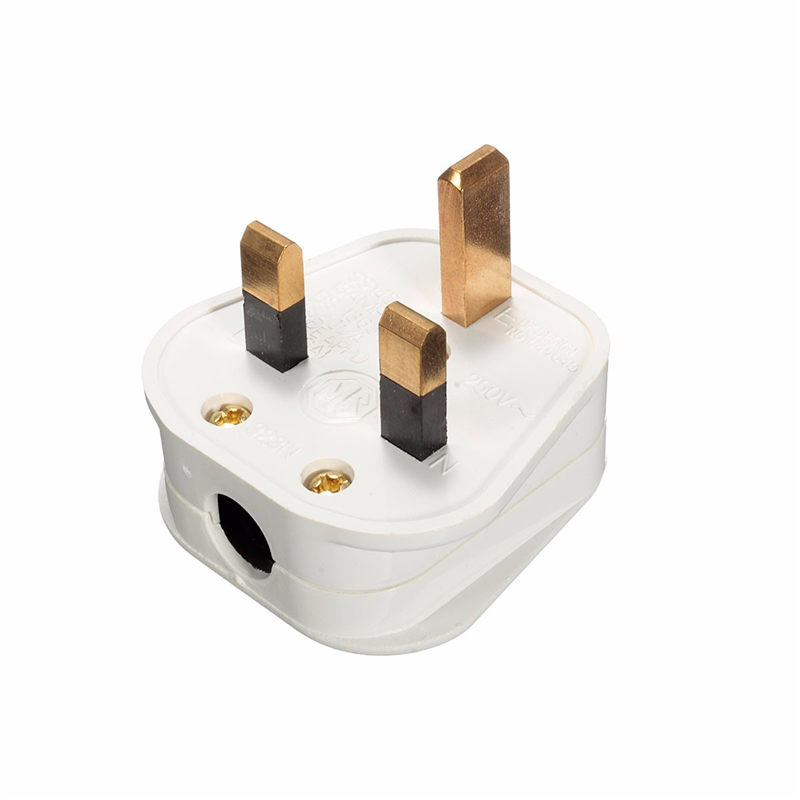
\includegraphics[scale=0.19]{13amp.jpg}\textbf{13 Amp:} This is your standard plug/cable that you use to power laptops, desk lamps, iPhone chargers. In the Students' Association we use it to provide power on stage, charge laptops during conferences as well as to get power to our sound and lighting desks, projectors, etc.  

\item 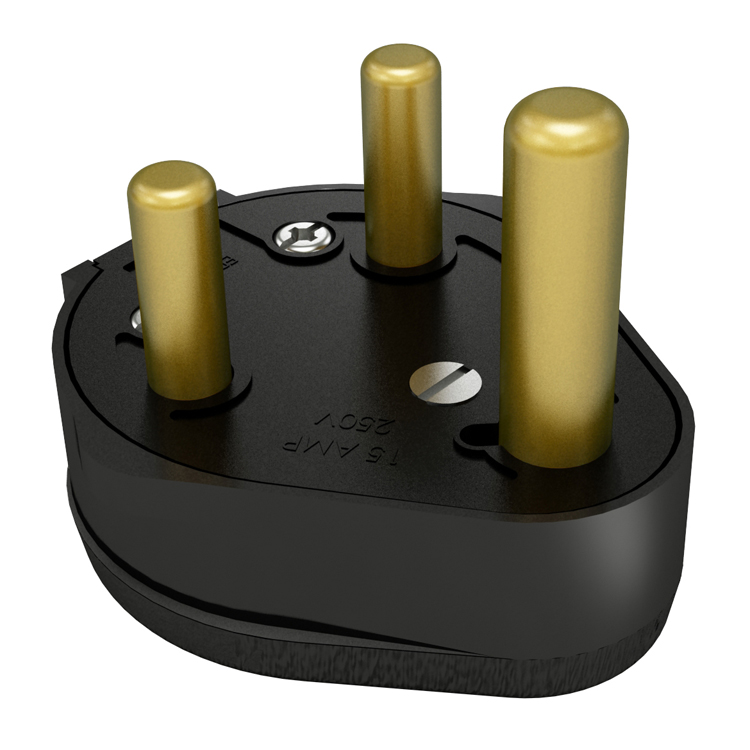
\includegraphics[scale=0.15]{15amp.jpg}\textbf{15 Amp:} This cable is almost exclusively used to power lights on a lighting rig. More detail is provided in the \textbf{Lighting Training}. 

\item 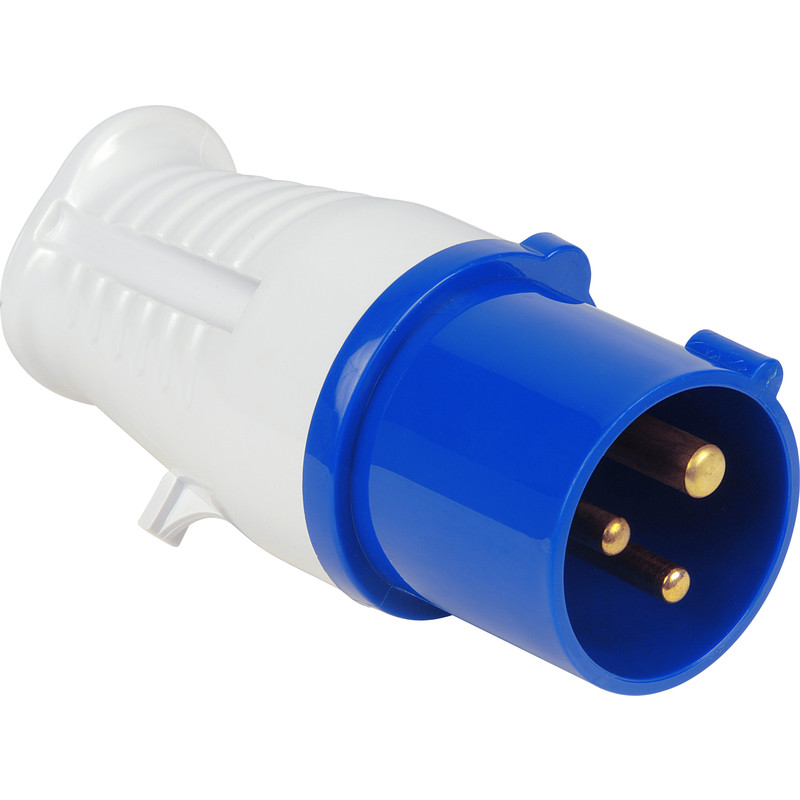
\includegraphics[scale=0.16]{16amp.jpg}\textbf{16 Amp:} This cable is widely used for different applications that require more power that what a 13 Amp cable can provide. The 16 Amp plug, unlike the 13 Amp one, can be used to provide power in an outside environment as it is waterproof. 

\item 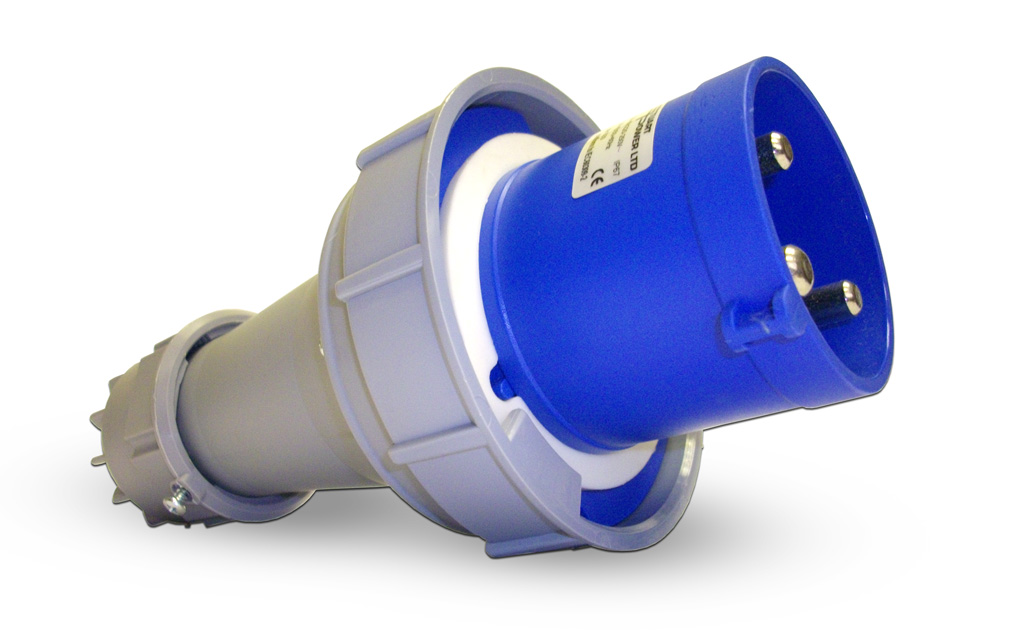
\includegraphics[scale=0.16]{32amp.jpg}\textbf{32 Amp:} This is a huge power plug that is used to provide even more power. They are often plugged into \textbf{Power Distribution Boxes}, which have multiple 16 Amp (or lower) sockets. 

\item 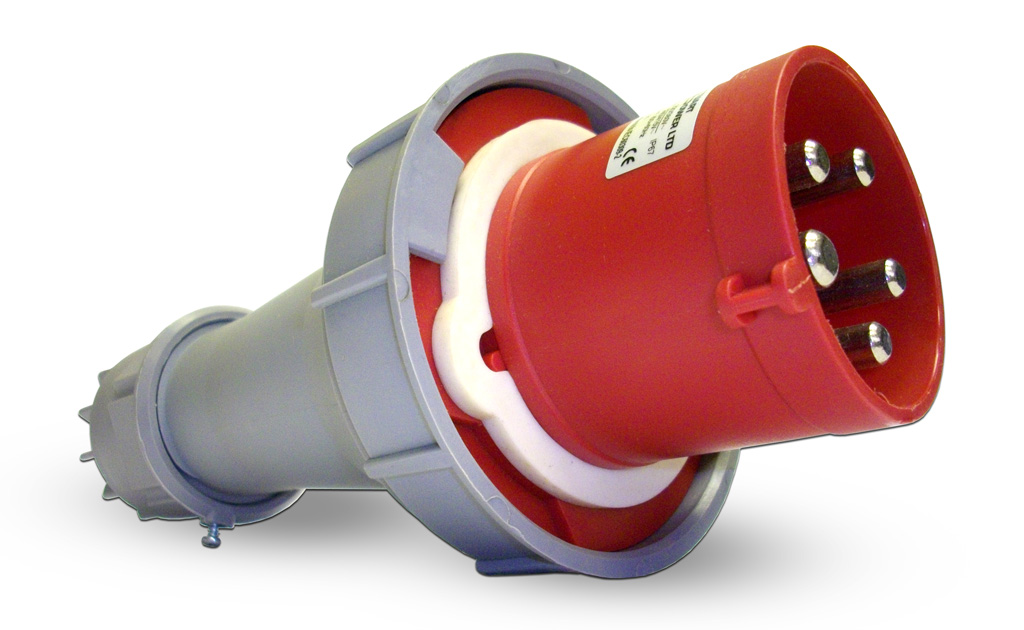
\includegraphics[scale=0.16]{63amp.jpg}\textbf{63 Amp:} Similar to 32 Amp, but huger and can provide even more power. Additionally, a 63 Amp cable can carry three-phase electrical power. 

\end{itemize}


\section{Introdution to Sound and Audio Systems}
\label{intro-sound}
In physics, \textbf{sound} is a vibration that propagates as a typically audible mechanical wave of pressure and displacement, through a transmission medium such as air or water. Humans can hear sound waves with frequencies \textbf{between about 20 Hz and 20 kHz}. Sound above 20 kHz is called \textbf{ultrasound} and below 20 Hz is called \textbf{infrasound}.

Sound by itself can be very loud. If you do not believe that, visit a kindergarden at launch break. However, it is often not loud enough. To help mititgate this problem we use a \textbf{Sound Reinforcement System}. 

\subsection{Structure of a Sound Reinforcement System}
\label{sound-system-structure}
A \textbf{Sound Reinforcement System} is the combination of microphones, signal processors, amplifiers, and loudspeakers in speaker cabinets that makes live or pre-recorded sounds louder and may also distribute those sounds to a larger or more distant audience. Such systems can range from very basic setups with a single microphone and/or music source up to massive line array systems with digital mixing desks and dozens of inputs. In general, though, the same principles apply to all of these systems, which helps to simplify them. A diagram of a typical sound reinforcement system is presented on Figure \ref{fig:intro}.

\begin{figure*}[h]
\begin{center}

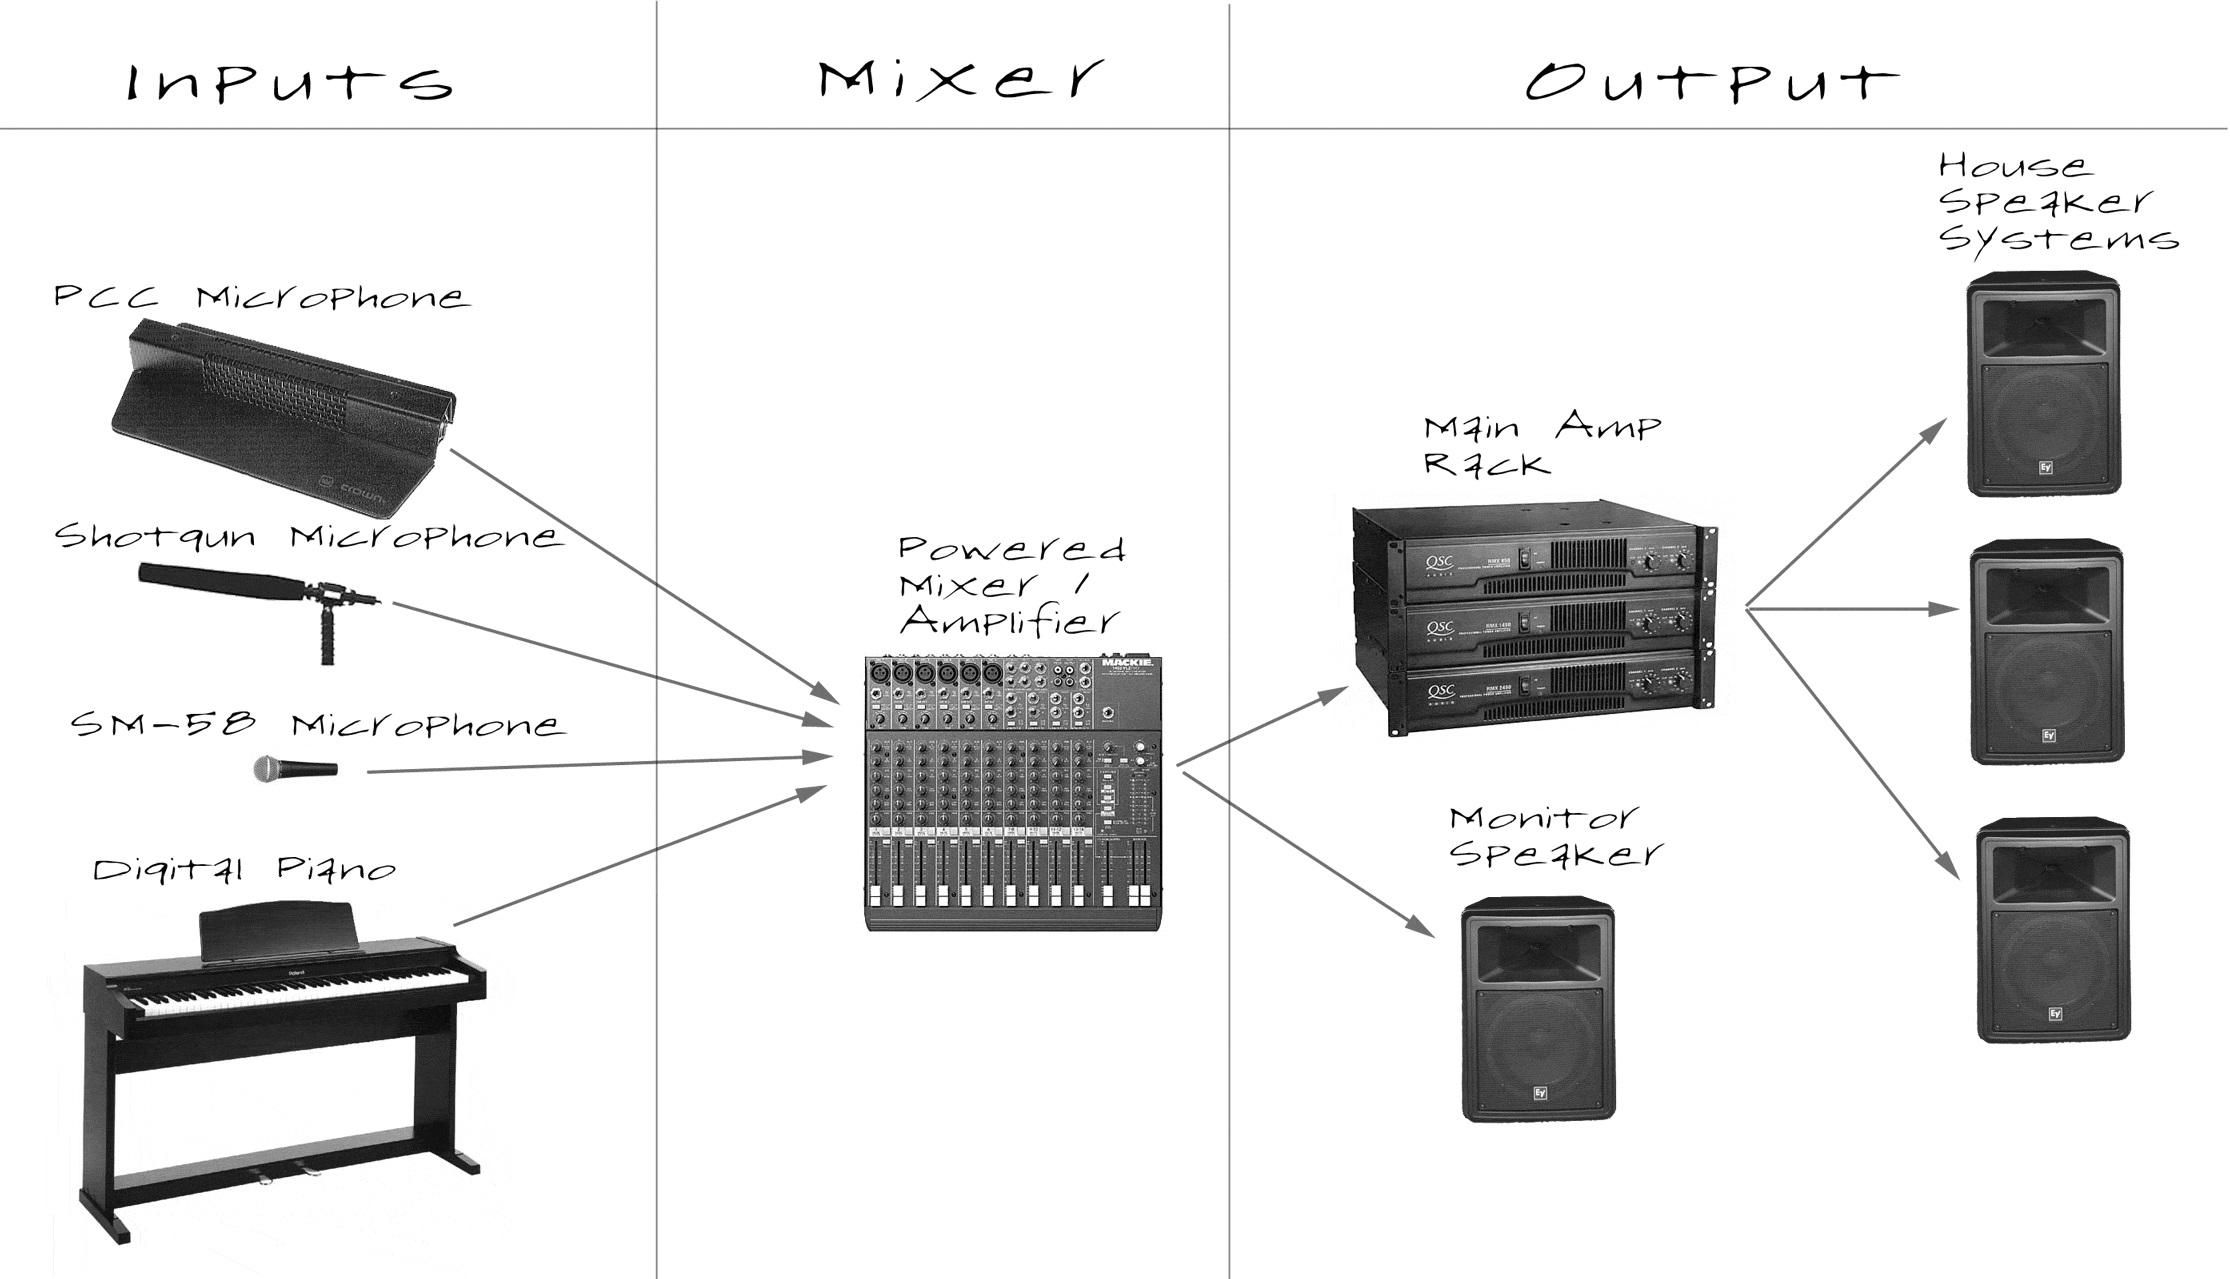
\includegraphics[width=18cm]{audio_labeled_diagram.jpg}
\caption{Basic structure of a sound system.}
\label{fig:intro}

\end{center}
\end{figure*}

The \textbf{INPUTS} section contains the different sources – basically anything that can make noise. We have to deal with a variety of sources, e.g. CD players, laptops, iPods, Microphones, DI boxes, etc. These all behave in slightly different ways which you will come across over time.

Then there is the \textbf{MIXER} section - it is possible to pass sound without a mixer, but then we have little or no control over it. Because we want to be able to combine signals together, the mixer is essential to creating an evenly balanced sound. They can also provide us with ways to route the signal to different sets of outputs (for example when mixing monitors for bands). Mixers, also called Mixing Desks, will be covered in more detail further on.

The first element in the \textbf{OUTPUT} section is the \textbf{power amplifier}. It increases the amplitude of the audio signal coming out of the mixer. Power amplifiers come in different shapes, sizes and power ratings. Last in the chain, after the amplifier, we have the \textbf{speakres} which turn the electrical signals from the amplifier into
sound waves. Speakers come in many flavours – some cover specific frequencies (e.g. subwoofers, or subs, which are designed to provide low frequency noise), some are designed to cover wide angles, while others are very directional. Speaker design is a bit of a dark art and there are some fascinating things that can be done!

It is worth noting that sometimes these elements can be combined together – sometimes you get mixers with built-in amplifiers (these are called powered mixers, we do not have any of these, but you may come across them), or more commonly, speakers sometimes have the amplifiers built in (these are called active speakers. If the amplifier is separate, it is a passive speaker.) The small Monacor PAs that we give to societies have a mixer, amplifier and speaker all built into one box. They are very neat, but generally less useful for our purposes!

\subsection{Signal Types}
\label{signal-types}
The electrical signals that travel through sound equipment come in a variety of sizes.
There are four main signal levels that you will need to know and understand. These are:

\begin{itemize}

\item \textbf{Microphone Level} - This is the level at which signal is sent out of a microphone. Because this is only voltage created by the movement of a coil within a microphone, it is very weak and therefore needs to be amplified using a pre-amp.

\item \textbf{Line Level} - This is the level at which professional audio equipment (CD players, mixing desks, DJ mixers, etc) outputs signal. It is much more powerful than microphone level and can be fed straight into an amplifier.

\item \textbf{Phono Level} - This is the level at which signal is generated by vinyl record decks as the needle bounces along the grooves of the record – it is a bit louder than microphone level, but still a long way from line level. Such signals have a
slightly stronger bass due to the mechanics of how they are generated. To compensate for this, they require special phono preamps which are built into most DJ mixers and some domestic hifi systems. It is not possible to connect them to other inputs, and if you connect a line level source to a phono preamp, it will sound distorted.

\item \textbf{Speaker Level} - This is the level at which amplifiers send out signal to speakers. It has to be powerful enough to make the speaker cone move and so is much more powerful than either microphone, line or phono levels.

\end{itemize}


\subsection{Balanced and Unbalanced Signals}
\label{balanced-unbalanced}
As sound signals tend to be very small electrically-speaking, they are susceptible to interference from external sources (e.g. radio waves, electromagnetic sources like power cabling, lighting transformers etc). This usually manifests as a buzz, or as other noises, especially over a long cable. Balancing offers an efficient solution to this. Knowing the exact theory is not necessary, but it is very interesting. 

If you take a signal cable, and you introduce a source of interference, you end up with the same interference acting roughly equally on all the cores of the cable. This interference is then amplified by the preamps and amps in a system until it’s audible, as shown on Figure \ref{fig:dirty-signal}.

\begin{figure*}[h]
\begin{center}

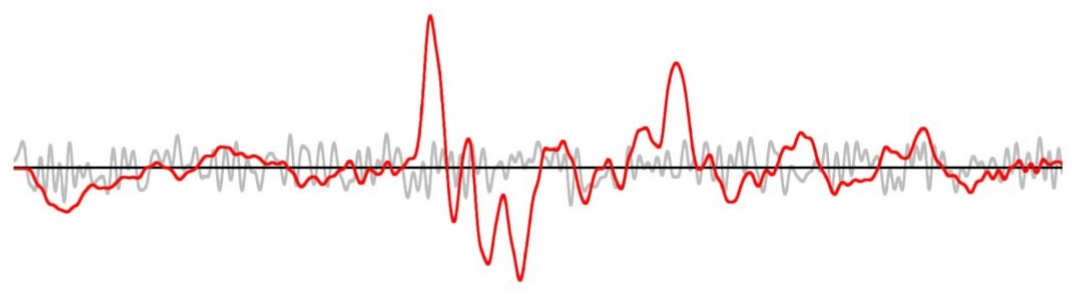
\includegraphics[width=18cm]{dirty-signal.png}
\caption{An image of a signal (shown in red) with some interference (shown in grey).}
\label{fig:dirty-signal}

\end{center}
\end{figure*}

Balancing involves sending an inverted signal along an adjacent cable core. This means that the same interference affects both signals, as shown on Figure \ref{fig:inverted-signal}.

\begin{figure*}[h]
\begin{center}

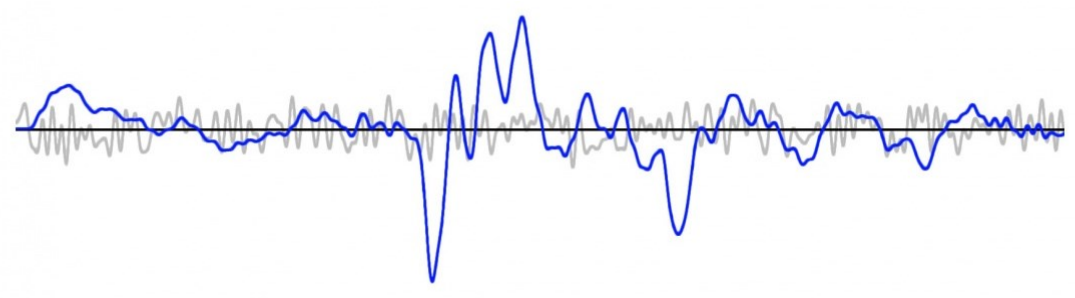
\includegraphics[width=18cm]{inverted-signal.png}
\caption{An image of the inverted signal (shown in blue) with the same interference (shown in grey).}
\label{fig:inverted-signal}

\end{center}
\end{figure*}

At the other end of the cable, the blue signal core gets inverted again, which flips both the signal and the interference, as shown on Figure \ref{fig:second-inverted}.

\begin{figure*}[h]
\begin{center}

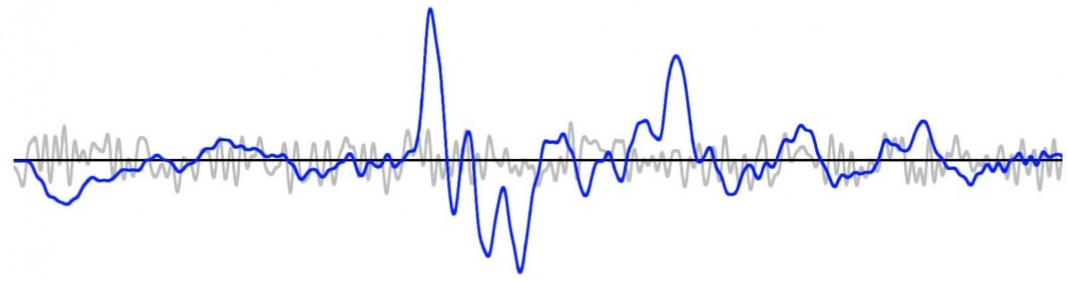
\includegraphics[width=18cm]{second-inverted.png}
\caption{An image of the re-inverted signal (shown in blue) with the now inverted interference (shown in grey).}
\label{fig:second-inverted}

\end{center}
\end{figure*}

If both the red and blue signals are added together, an even stronger version of the original signal is produced and the interference is canceled out, as shown on Figure \ref{fig:clean-signal}. This is a balanced signal. 

\begin{figure*}[h]
\begin{center}

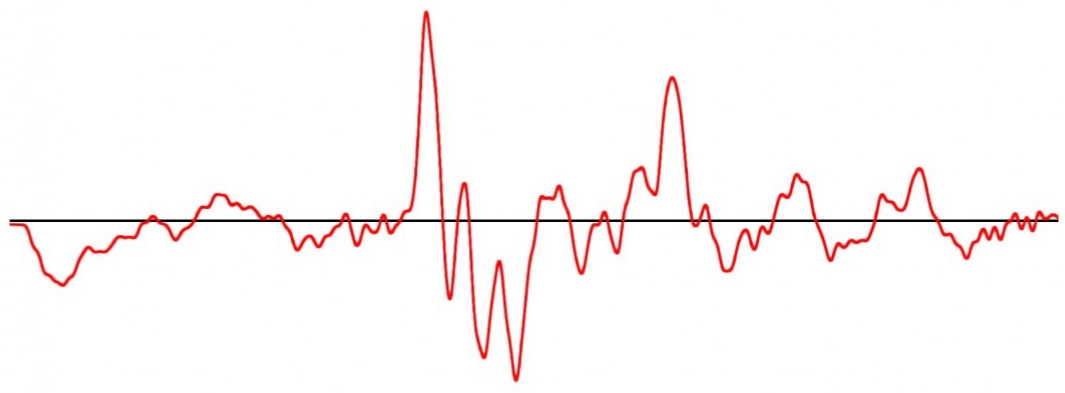
\includegraphics[width=18cm]{clean-signal.png}
\caption{An image of the produced stronger clean signal (shown in red) with no interference.}
\label{fig:clean-signal}

\end{center}
\end{figure*}

Thus a balanced signal is far less susceptible to noise and interference than an unbalanced signal.

\subsection{Balanced and Unbalanced Cables}
\label{balanced-unbalanced-cables}
As there are balanced and unbalanced signals, there are also balanced and unbalanced cables, i.e. cables that carry balanced and unbalanced signals, respectively.

A cable carrying \textbf{unbalanced signal} needs two connectors - one of these is "ground" and the other carries the signal.

A cable carrying \textbf{balanced signal} needs three connectors - ground, signal and an inverse copy of the signal. All the connecturs are wrapped around each other so that the external noise can affect them equally. 


\subsubsection{Balanced Cables}
\label{balanced-cables} 
There are two types of balanced cables that you will encounter in the Edinburgh University Students' Association:

\begin{itemize}

\item 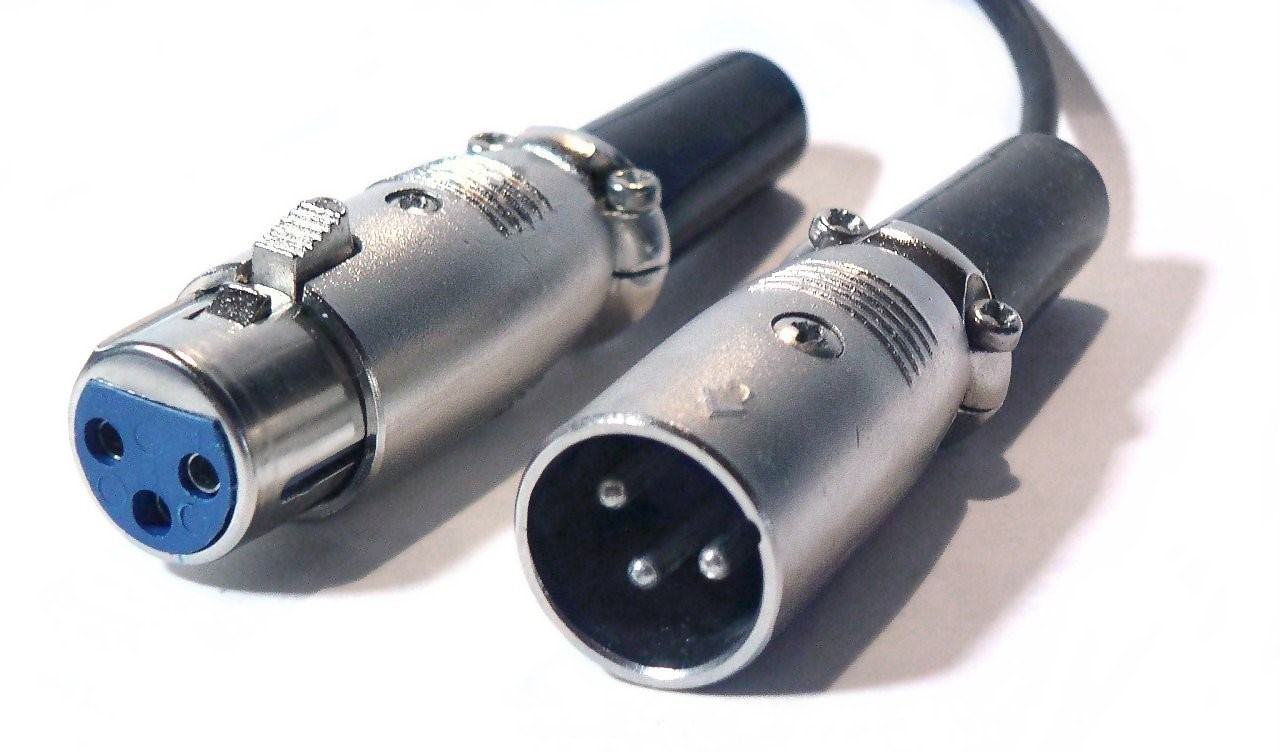
\includegraphics[scale=0.12]{xlr2.jpg}\textbf{XLR:} This is the most common type of cable in the sound world. Frequently referred to by musicians as "mic cable". Has three pins/holes.

\item 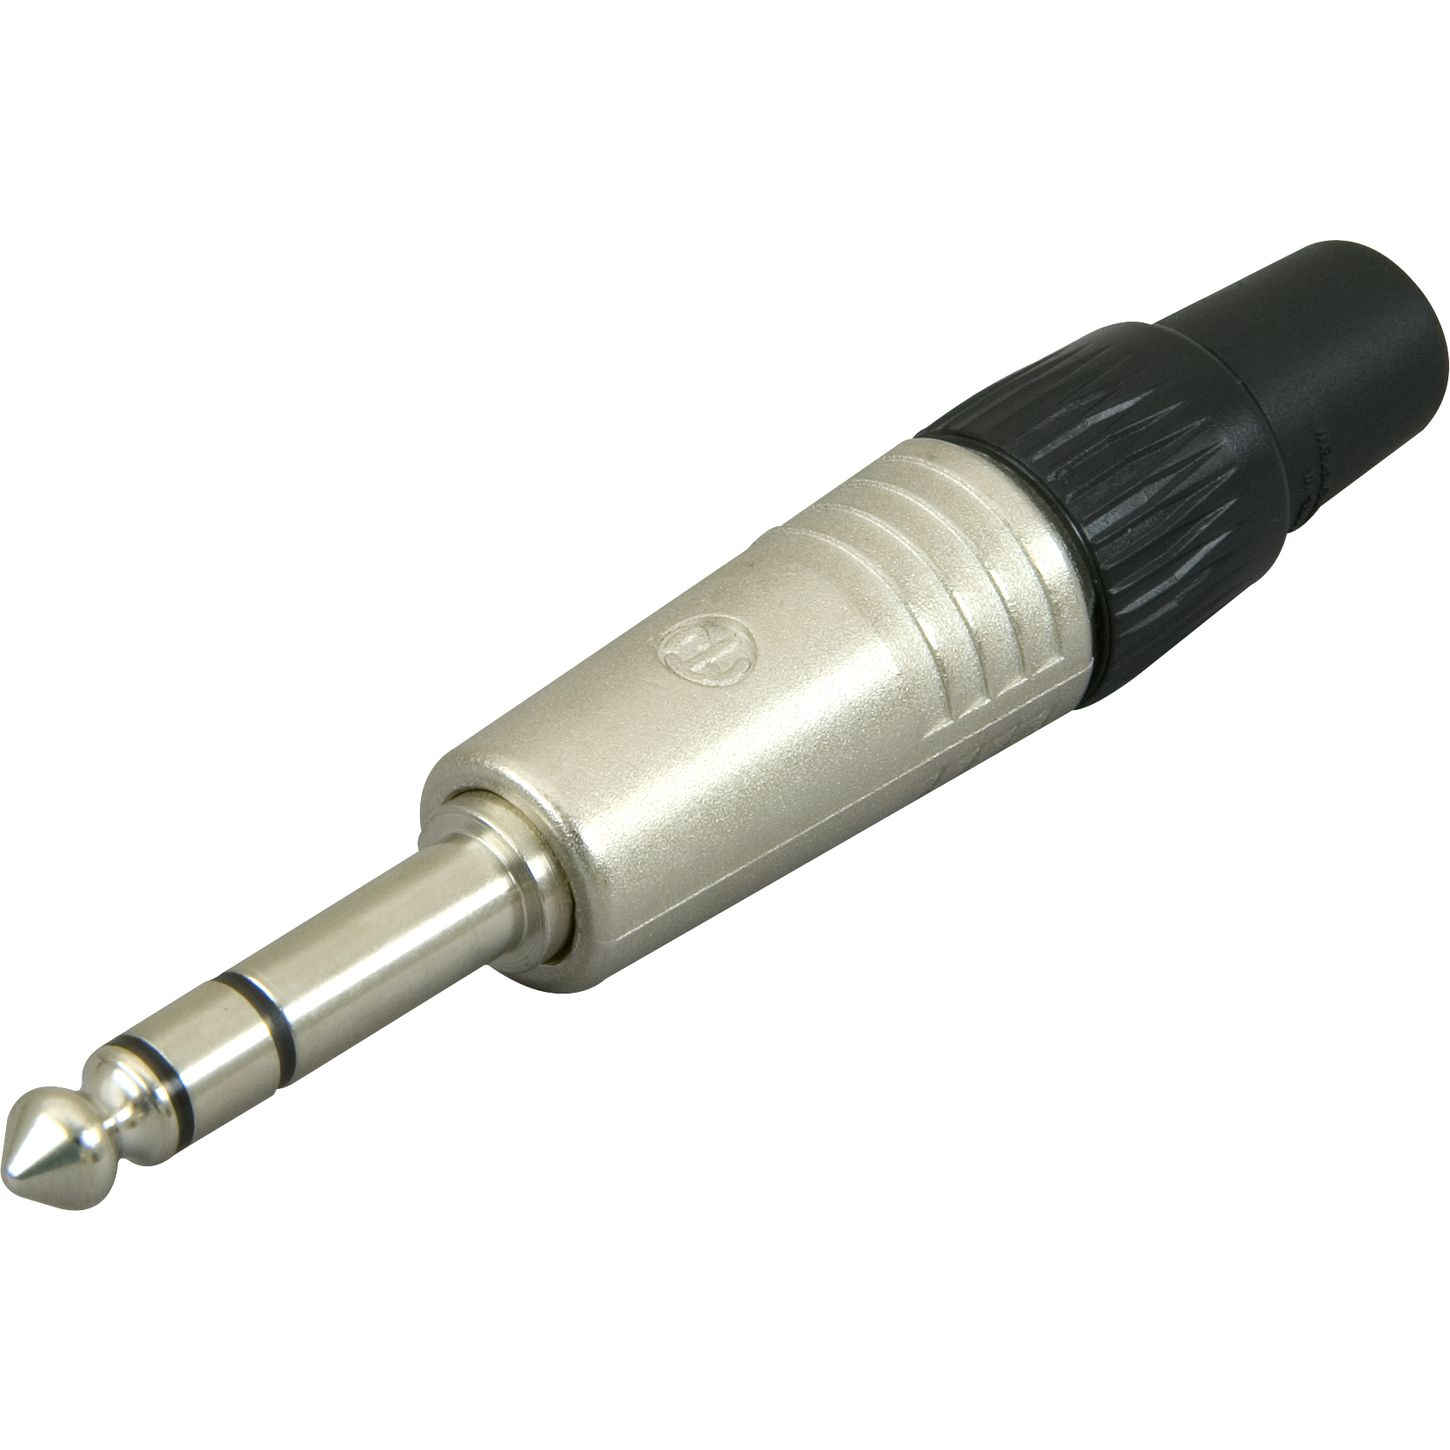
\includegraphics[scale=0.35]{bal_jack.jpg}\textbf{Balanced Jack (TRS):} This has three connections: tip, ring and sleeve. It is explained in more detail in the \textbf{Sound Training}. Not to be confused with unbalanced jack (guitar cable).

\end{itemize}


\subsubsection{Unbalanced Cables}
\label{unbalanced-cables} 
There are three types of unbalanced cables that you will encounter in the Edinburgh University Students' Association:


\begin{itemize}

\item 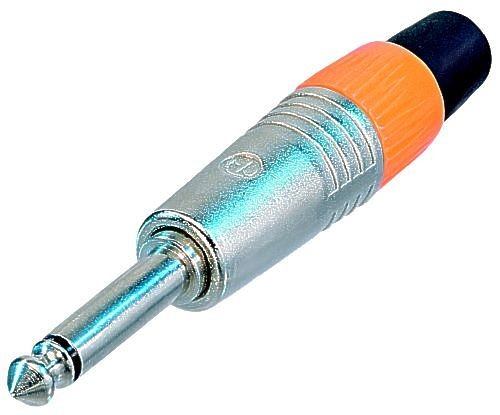
\includegraphics[scale=0.22]{jack_ts.jpg}\textbf{Unbalanced Jack (TS):} This has two connections: tip and sleeve. This is a guitar cable, do not confuse it with balanced jacks! Commonly known as 6.35mm or 1/4inch jack.

\item 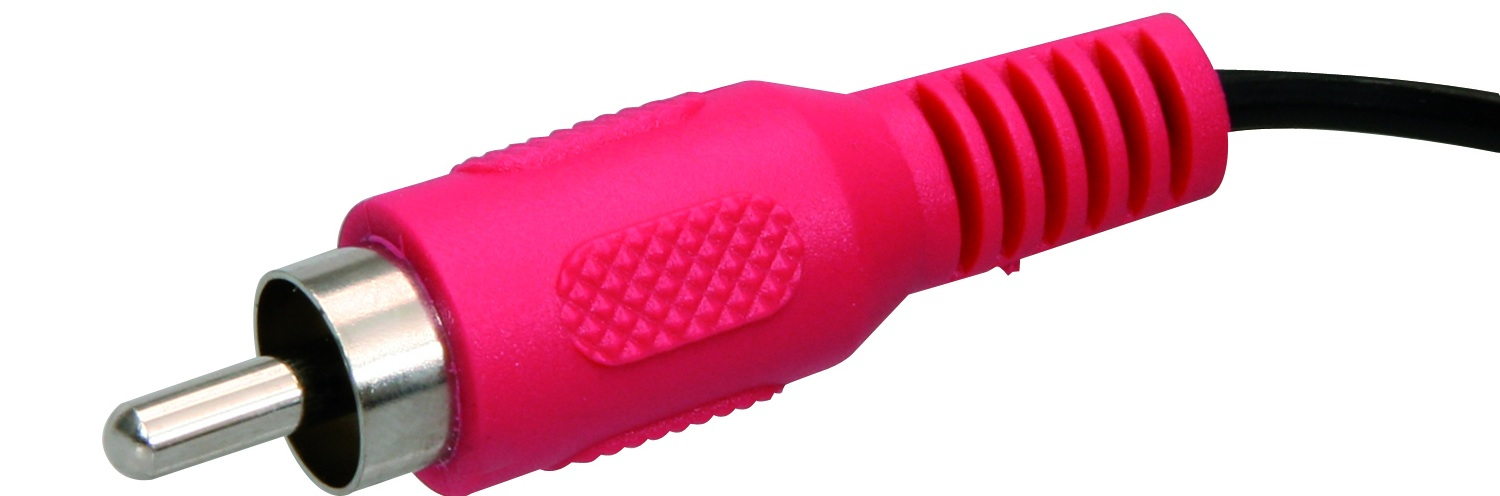
\includegraphics[scale=0.11]{rca.jpg}\textbf{RCA:} This is commonly used by DJ equipment, CD players, hi-fi types. Frequently referred to as "phono cable".

\item 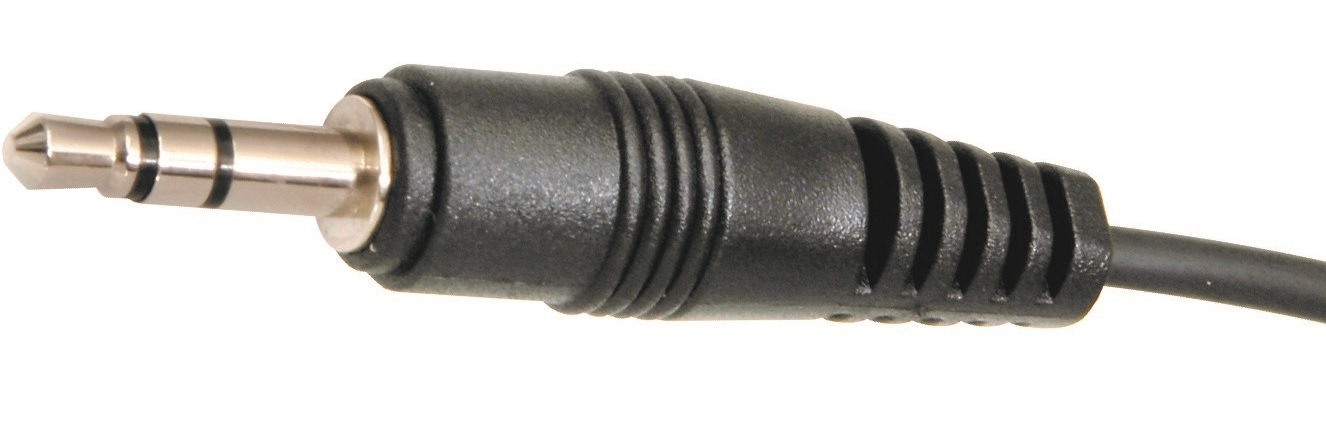
\includegraphics[scale=0.2]{minijack2.jpg}\textbf{Minijack:} This is used by laptops, iPods and other consumer equipment. Commonly referred to as an "aux cable", "3.5mm jack" or "Hi, can I play my laptop through your speakers?". Enjoys popping out mid-gig. Note that, while there are three connectors, it is unbalanced. This is because it carries stereo (two channel) signal. 

\end{itemize}

\subsubsection{Speaker Cables}
\label{speaker-cables} 
The previously presented cables carry microphone, line and phono level signals. However, cables are also needed to carry speaker level signals:

\begin{itemize}

\item 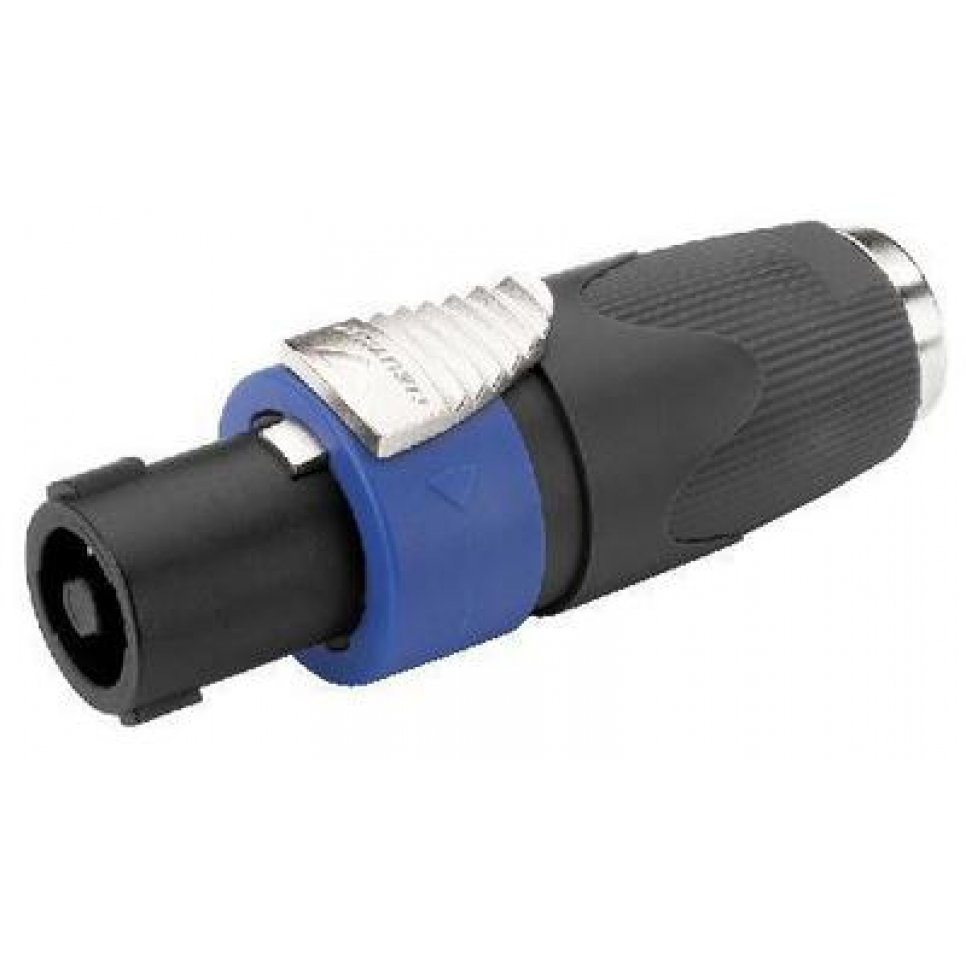
\includegraphics[scale=0.16]{nl2.jpg}\textbf{Speakon (NL2, NL4, NL8):} This is used to carry speaker level signal. Comes in several forms, with the number indicating the number of cores. The cores come in pairs, so NL2 can carry one signal, NL4 can carry two and NL8 can carry four signals.

\end{itemize}

\subsection{Mixing Desks}
\label{mixing-desks}
In audio, a \textbf{mixing console (mixing desk)} is an electronic device for combining (also called "mixing"), routing, and changing the volume level, timbre (tone color) and/or dynamics of many different audio signals, as produced by the devices presented in the \textbf{INPUTS} section of Figure \ref{fig:intro}. Figure \ref{fig:mixing-desk} provides a simple image of the workings of a mixing desk. Mixing desks can be either analogue or digital, depending on whether they work on analogue or digital audio signals. 

\begin{figure}[h]
\begin{center}

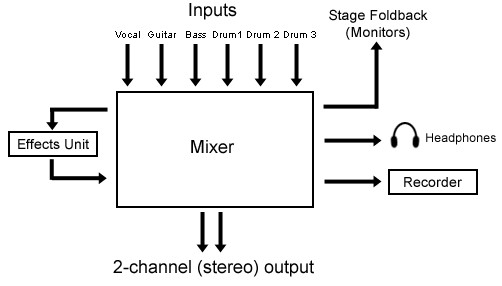
\includegraphics[width=9cm]{mixing-desk3.jpg}
\caption{A simple diagram of a standard mixing desk.}
\label{fig:mixing-desk}

\end{center}
\end{figure}

At the \textbf{Edinburgh University Students' Association} we have several mixing desks of different shapes and sizes. They are covered in more detail in the \textbf{Sound Training}. Here we use the \textbf{Midas Verona}, a.k.a. Matilda, as an example, as it is our most complex analogue desk. All analogue desks are based around the same concepts , although many remove or simplify a lot of the features. We shall now look at the two types of sections an analogue mixing desk has - \textbf{Channel Strip} and \textbf{Master Section}.


\subsubsection{Channel Strip}
\label{channel-strip}
A channel on a mixing desk is responsible for a single input, which could be a microphone, DI box, etc. Consequently, on analogue desks, the number of channels limits the number of inputs you can have. The cahnnel strip gives you control to change the amplitude of the input signal, change its sonic attributes and deside how it will be mixed along with the other channels. A detailed description of the channel strip is provided on Figure \ref{fig:channel-strip}.

\begin{figure}[h]
\begin{center}

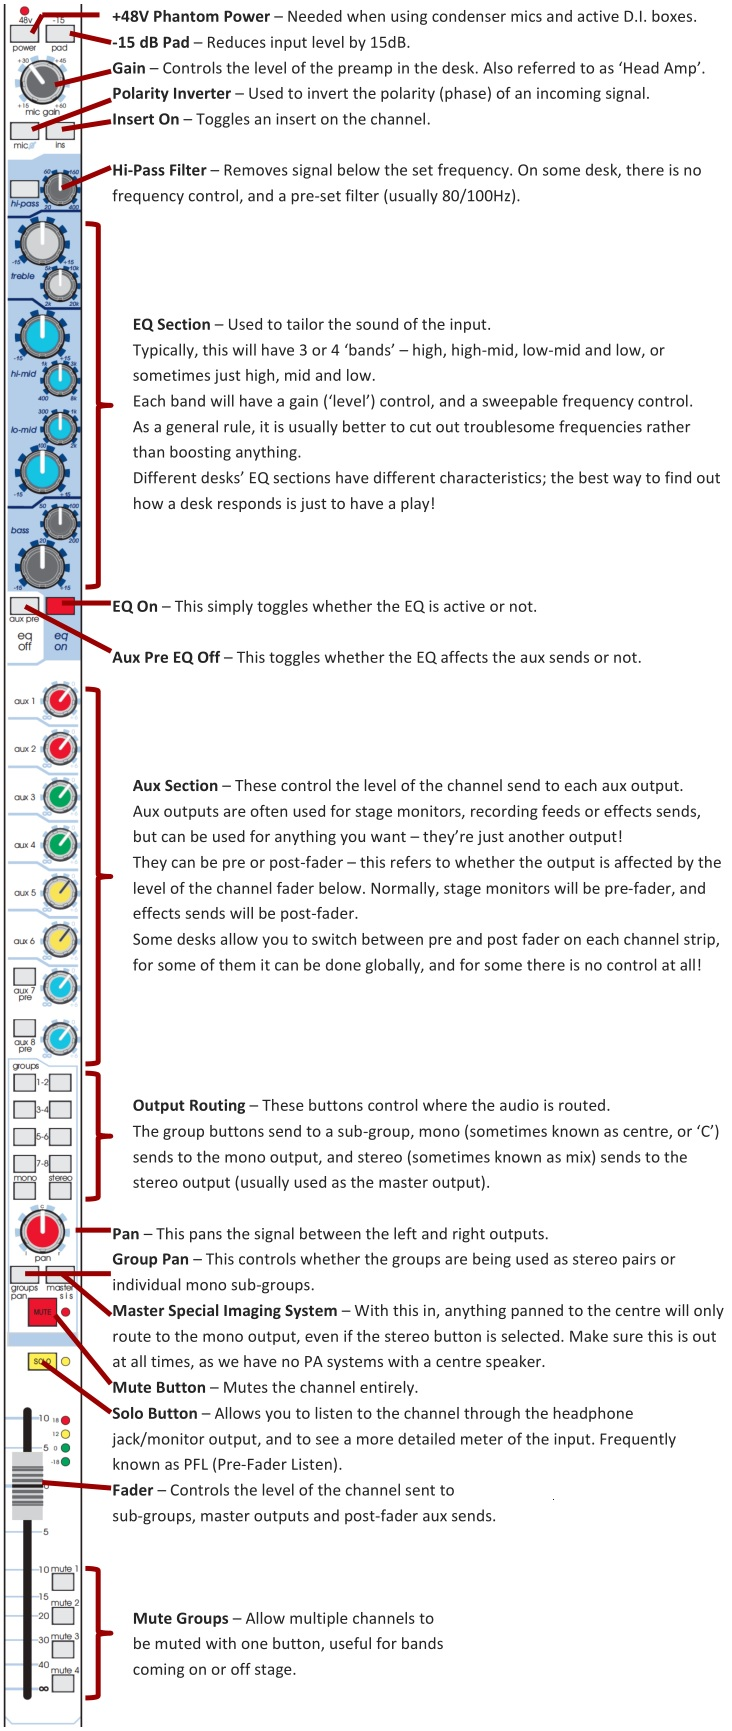
\includegraphics[width=10cm]{channel-strip.jpg}
\caption{An image of a standard mixing desk input strip.}
\label{fig:channel-strip}

\end{center}
\end{figure}

\subsubsection{Master Section}
\label{master-section}
The master section is where all the master volume controls for each output can be found. On the Midas Verona, it is separated into two parts - \textbf{Auxiliary (AUX) Master Section}, shown on Figure \ref{fig:aux-section}, and \textbf{Main Master Section}, shown on Figure \ref{fig:master-section}.

\begin{figure}[h]
\begin{center}

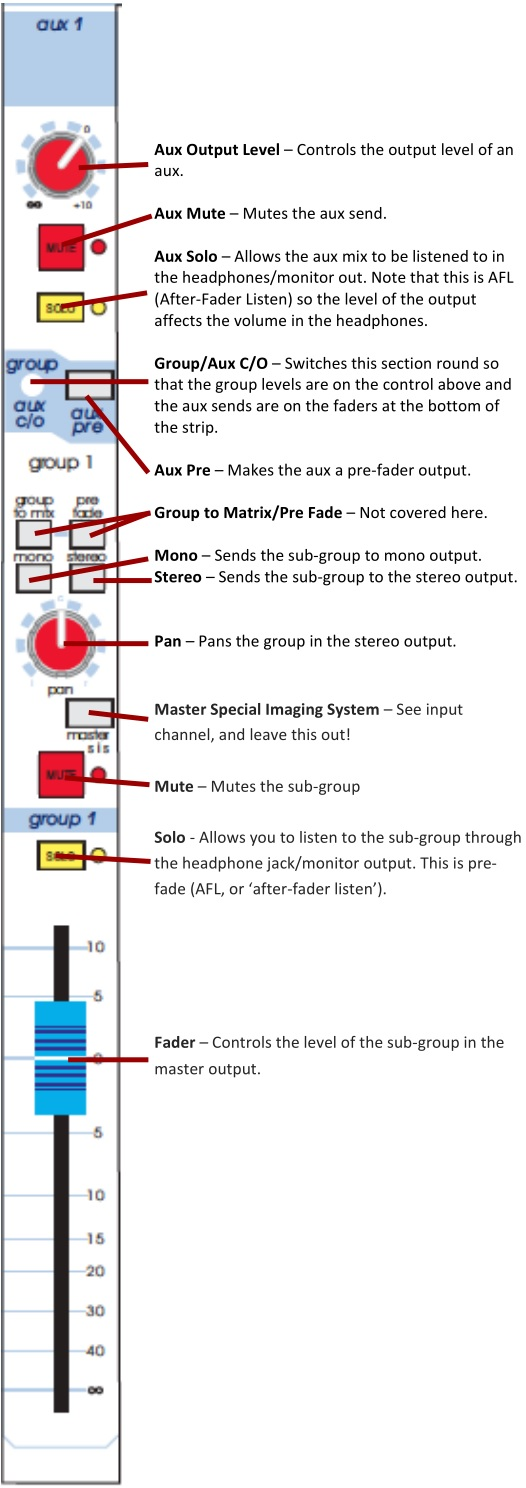
\includegraphics[width=8cm]{aux-section.jpg}
\caption{An image of the Auxiliary (AUX) Master Section.}
\label{fig:aux-section}

\end{center}
\end{figure}

\begin{figure}[h]
\begin{center}

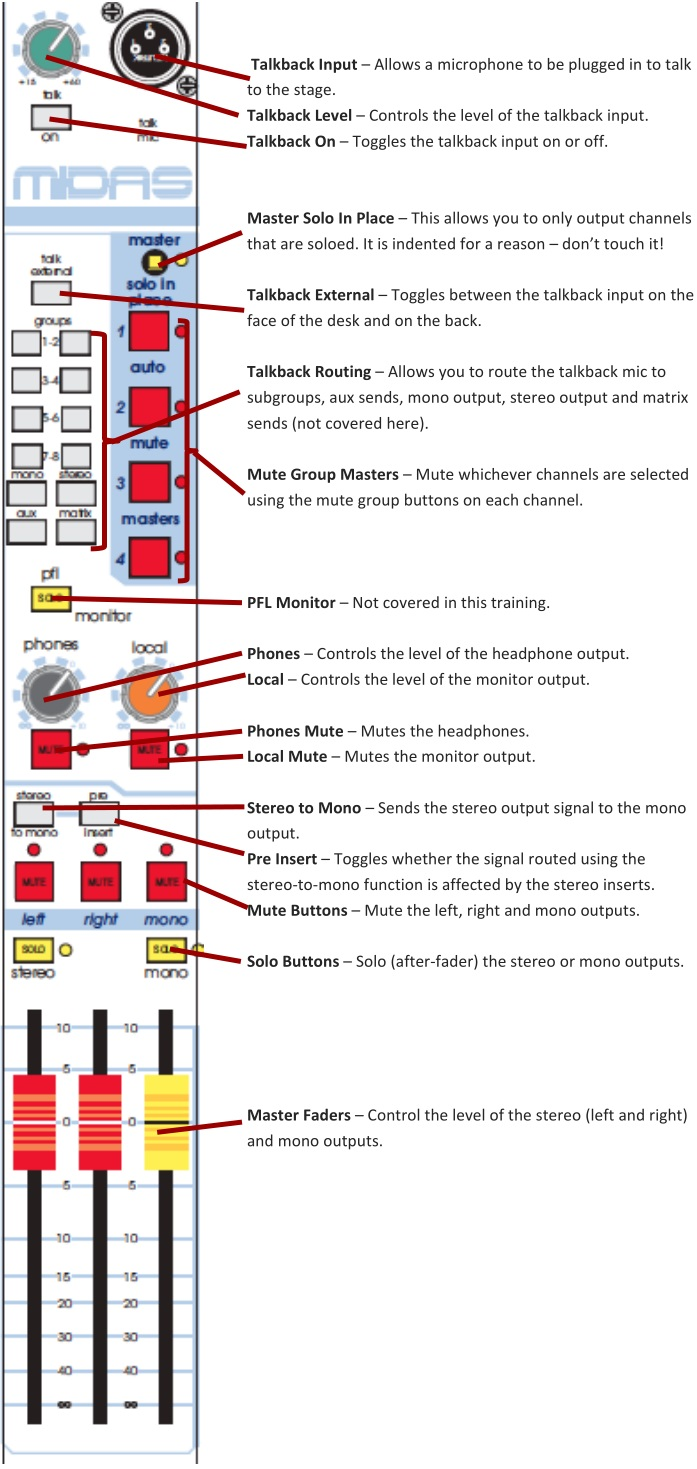
\includegraphics[width=10cm]{master-section.jpg}
\caption{An image of the Main Master Section.}
\label{fig:master-section}

\end{center}
\end{figure}


\section{Lighting}
\label{lighting}
Some sort of basic lighting training (if applicable). To be filled by the lampeys.

\section{AV}
\label{av}
To be filled as well.

\section{Conclusion}
\label{conclusion}
To be filled with some random stuff.

%\begin{figure}[h]
%\begin{center}
%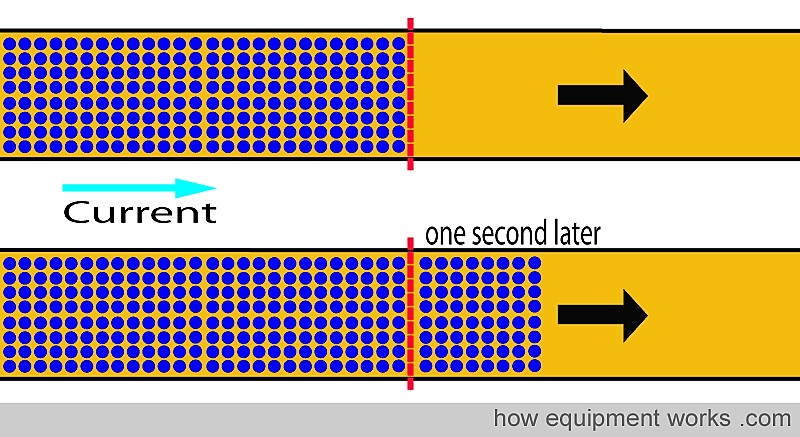
\includegraphics[width=9cm]{one-second-current2.jpg}
%\caption{The electrons passing through a cross section of the wire.}
%
%\label{fig:one-second-current}
%\end{center}
%\end{figure}

 



\end{document}

%----------------------------------------------------------------------------------------
%	ARTICLE CONTENTS
%----------------------------------------------------------------------------------------